\subsection{Itération n°4}

\subsubsection{Configuration, modifications et résultats attendus}

Nous avons une autre idée de la cause de ces résultats décevants. Il pourrait s'agir d'un manque d'exploration. Donc nous essayons d'utiliser un nombre bien plus grand d'épisodes. Nous prenons 800 cycles composés de 200 épisodes.

Nous espérons voir une décroissance de la perte de la critique et de la politique et une augmentation de la récompense. Si c'est le cas, alors le problème est effectivement un manque de données d'exploration. Si nous n'obtenons pas de résultats concluants nous nous pencherons sur une nouvelle implémentation d'algorithme par renforcement profond.

\subsubsection{Analyse}

\begin{figure}[H]
    \centering
    \begin{subfigure}{0.3\textwidth}
        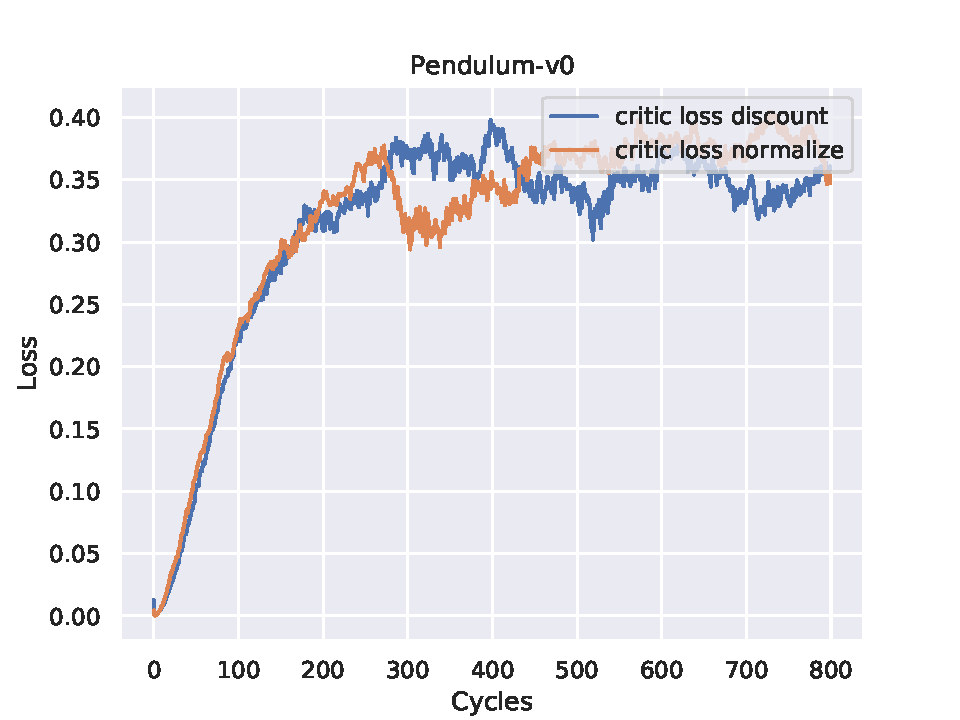
\includegraphics[width=\textwidth]{figures/iteration4/critic_loss_Pendulum-v0_pg_dataset_td_eval_True_cycles_800_trajs_200_batches_20_gamma_0.99_nstep_5_lr_act_0.01_lr_critic_0.01pg.pdf}
        \caption{Fonction de perte de la critique}
    \end{subfigure}
    \begin{subfigure}{0.3\textwidth}
        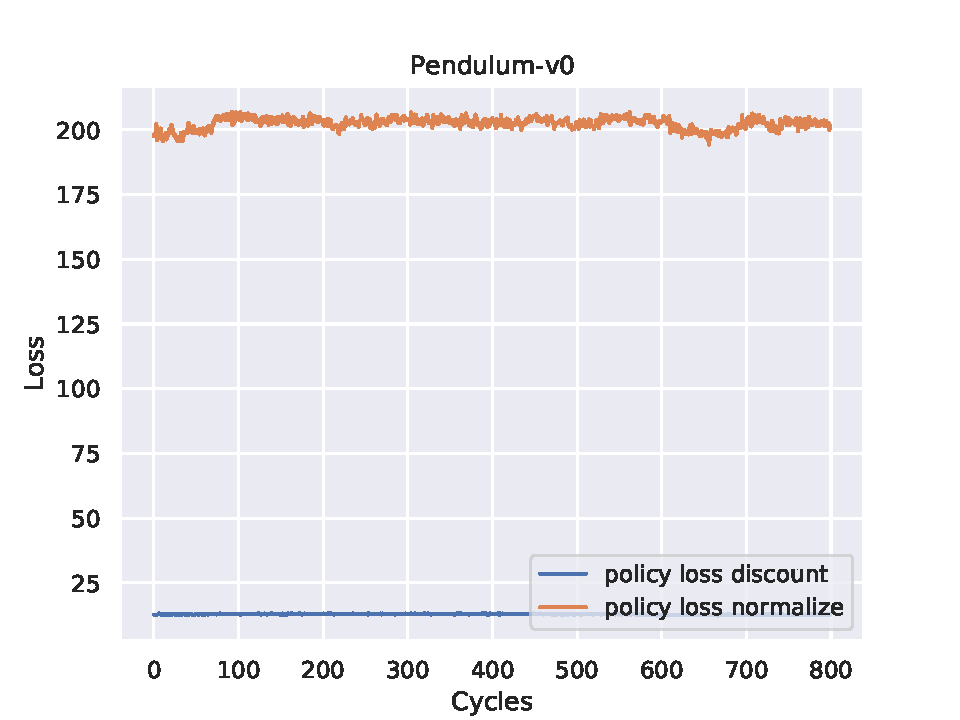
\includegraphics[width=\textwidth]{figures/iteration4/policy_loss_Pendulum-v0_pg_dataset_td_eval_True_cycles_800_trajs_200_batches_20_gamma_0.99_nstep_5_lr_act_0.01_lr_critic_0.01pg.pdf}
        \caption{Fonction de perte de la politique}
    \end{subfigure}
    \begin{subfigure}{0.3\textwidth}
        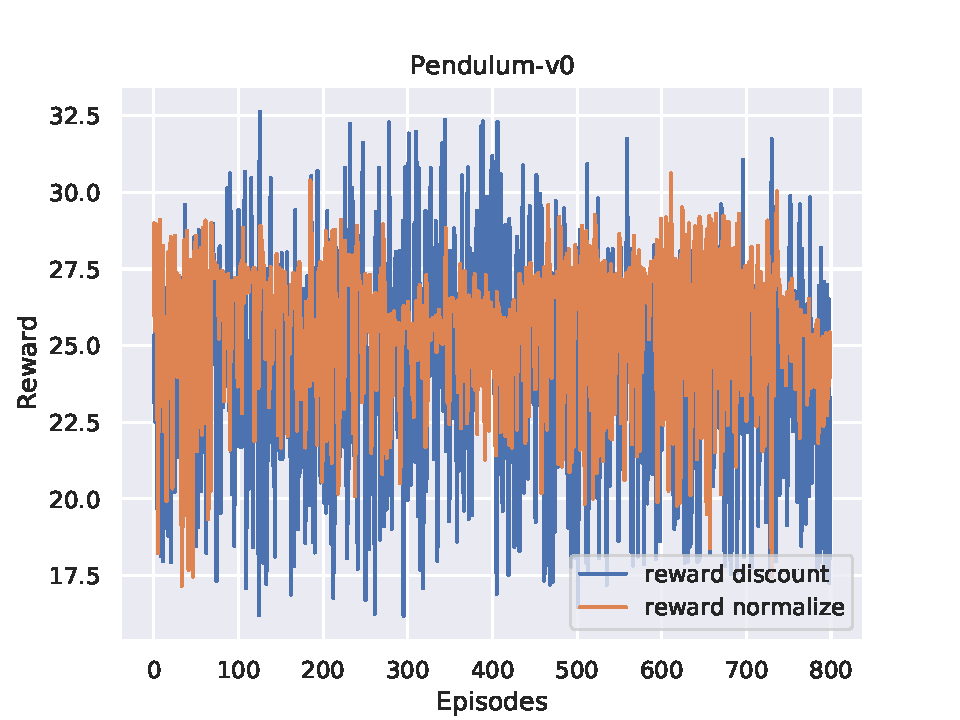
\includegraphics[width=\textwidth]{figures/iteration4/rewards_Pendulum-v0_pg_dataset_td_eval_True_cycles_800_trajs_200_batches_20_gamma_0.99_nstep_5_lr_act_0.01_lr_critic_0.01.pdf}
        \caption{Récompenses des épisodes}
    \end{subfigure}
    \caption{Résultats obtenus pour la critique, la politique et la récompense}
    \label{fig:itr4_results}
\end{figure}

Malgré l'augmentation de l'exploration et du nombre de trajectoire par \emph{batch}, les résultats obtenus sont très similaires et rien ne s'est amélioré. Nous attendons toujours que la fonction perte de la critique finisse par décroître. Le comportement singulier des pertes sur la politique nous interroge toujours autant. Enfin, la récompense n'a pas évoluer malgré le grand nombre d'itérations.

\begin{figure}[H]
    \centering
    \begin{subfigure}{0.3\textwidth}
        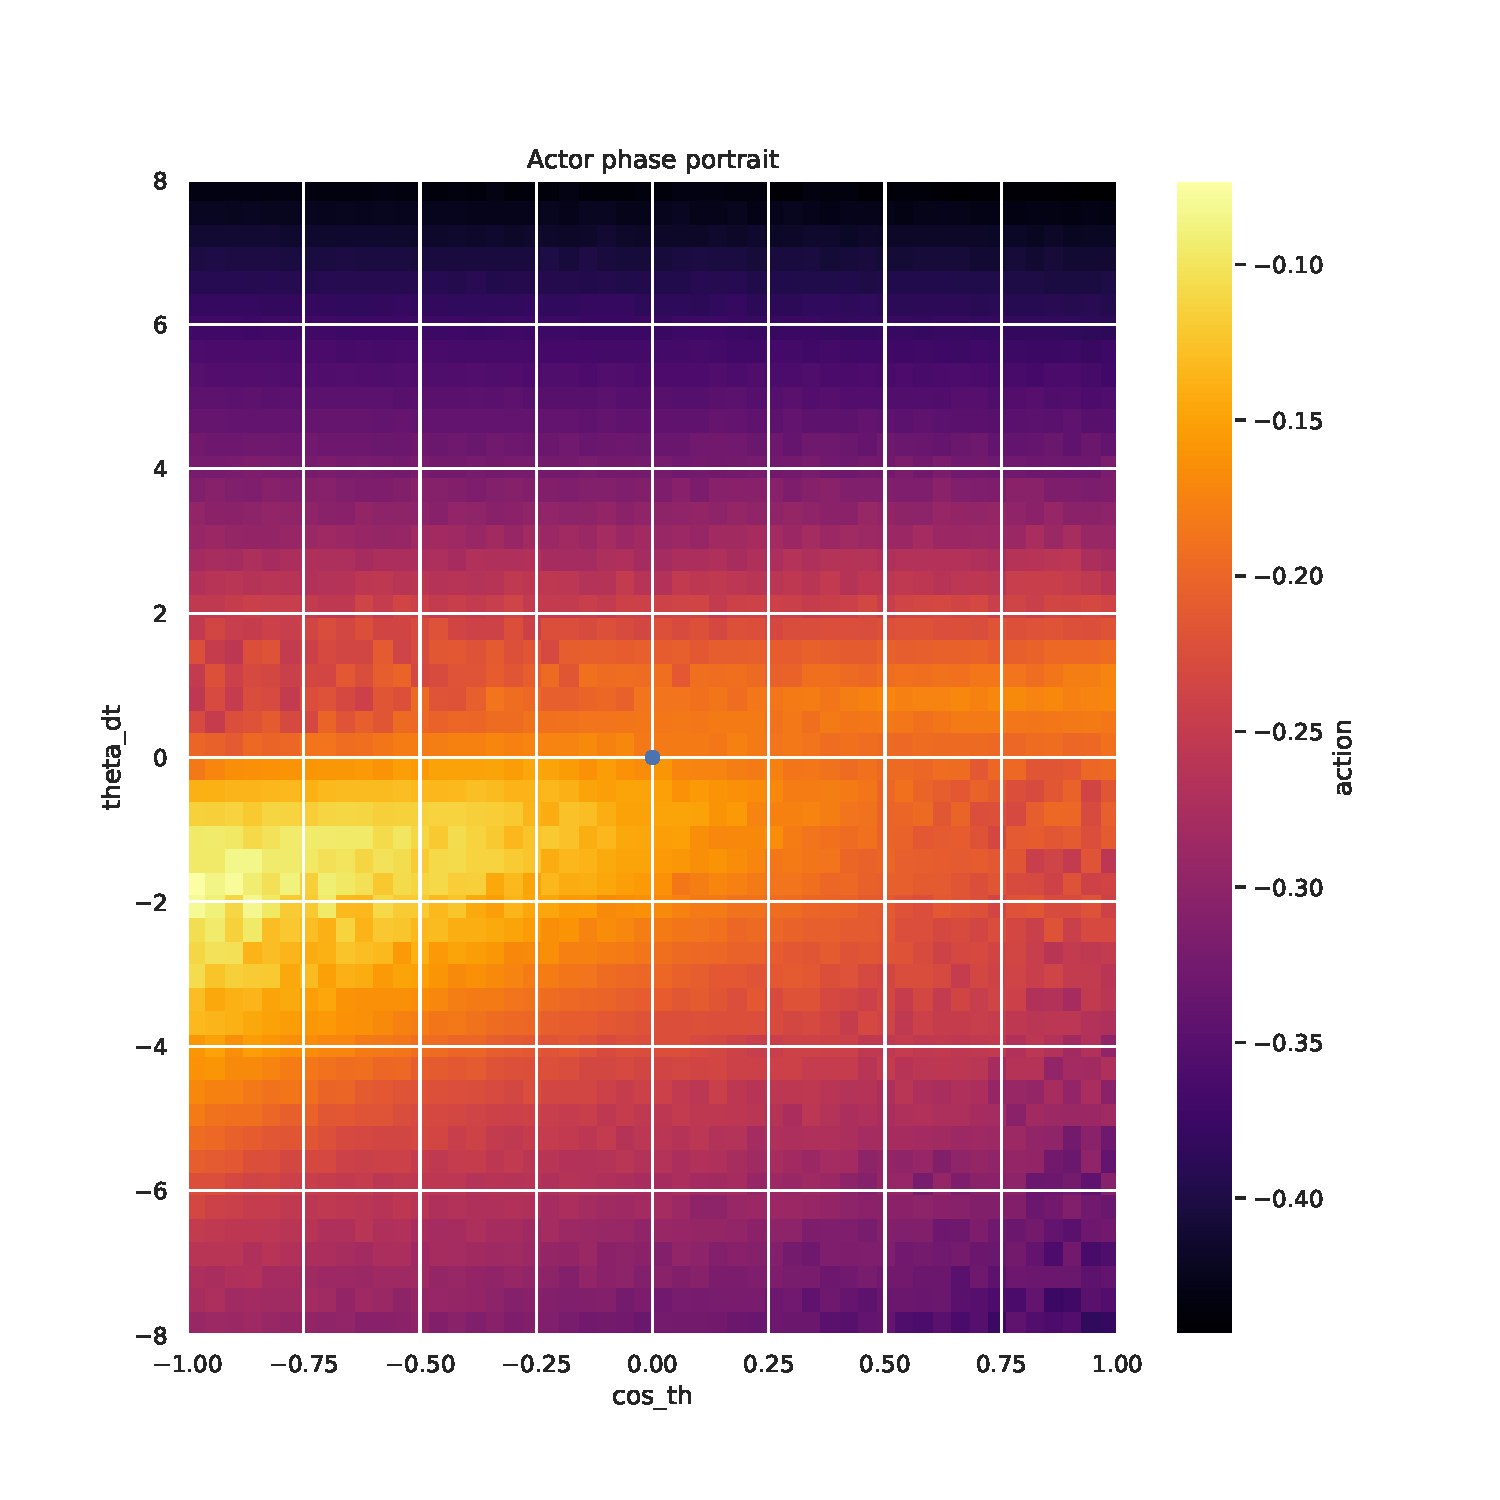
\includegraphics[width=\textwidth]{figures/iteration4/0_actor_discount__ante_Pendulum-v0.pdf}
        \caption{Acteur naïf}
    \end{subfigure}
    \begin{subfigure}{0.3\textwidth}
        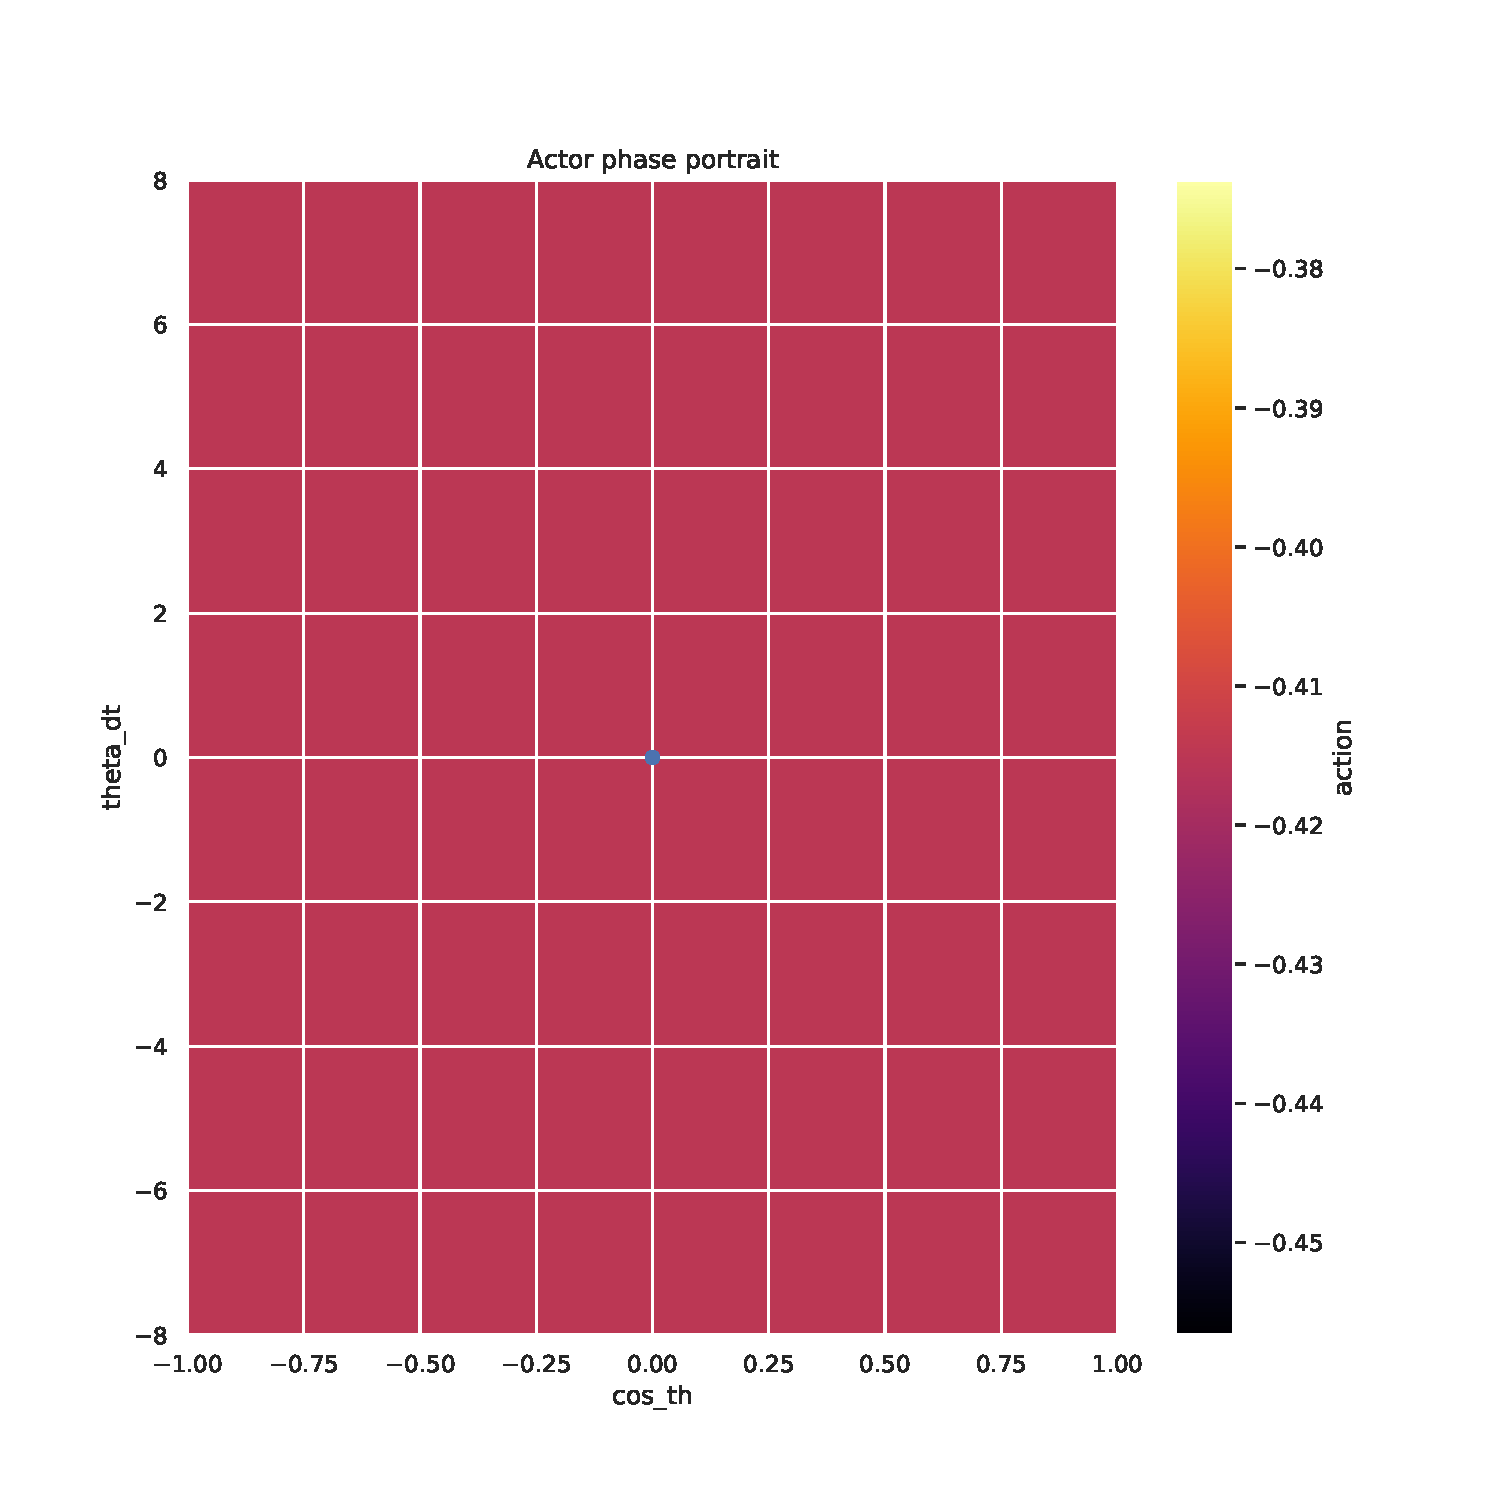
\includegraphics[width=\textwidth]{figures/iteration4/0_actor_discount__post_Pendulum-v0.pdf}
        \caption{Acteur entraîné}
    \end{subfigure}
    \begin{subfigure}{0.3\textwidth}
        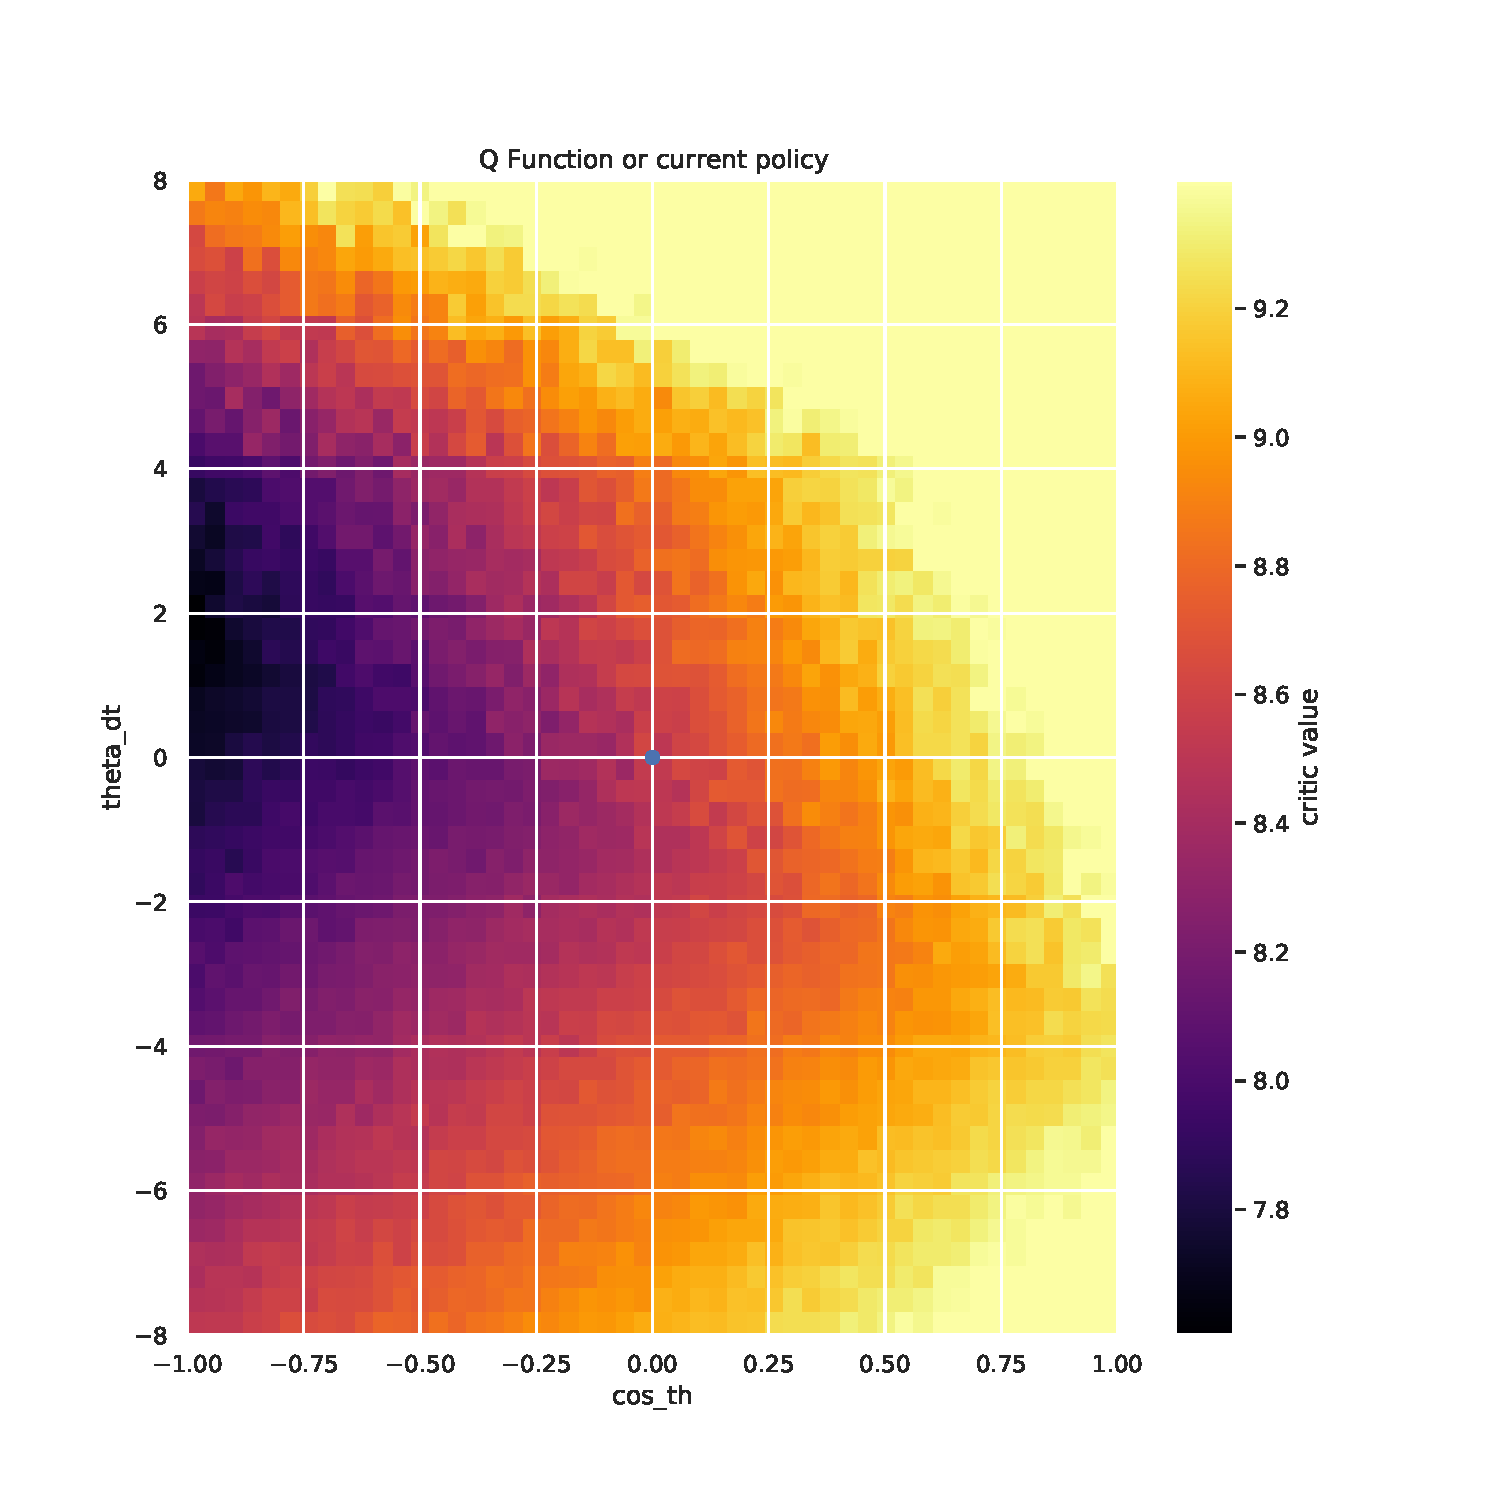
\includegraphics[width=\textwidth]{figures/iteration4/0_critic_discount_post_Pendulum-v0.pdf}
        \caption{Critique entraînée}
    \end{subfigure}
    \caption{Valeurs de l'acteur et de la critique avec la méthode discount pour le calcul de la récompense}
    \label{fig:itr4_discount}
\end{figure}

\begin{figure}[H]
    \centering
    \begin{subfigure}{0.3\textwidth}
        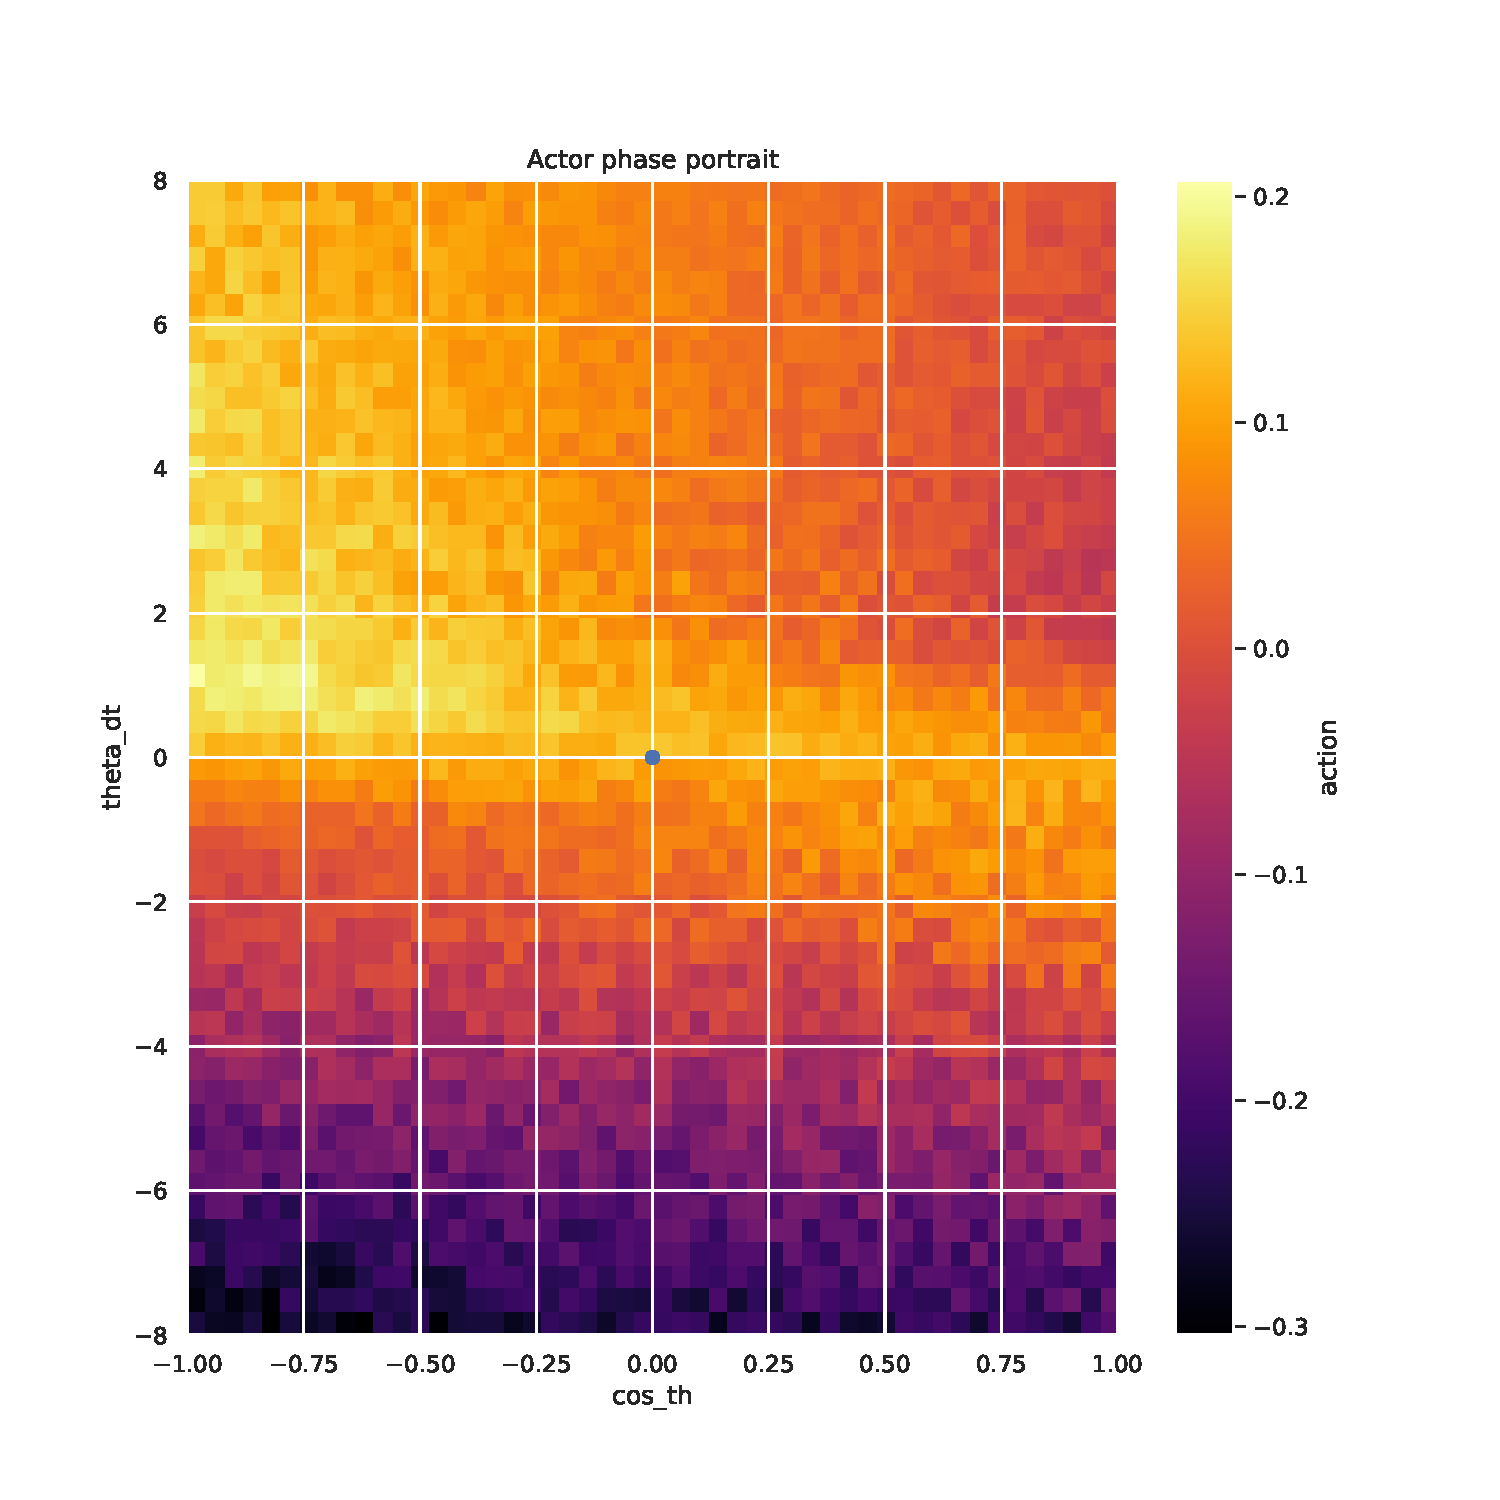
\includegraphics[width=\textwidth]{figures/iteration4/0_actor_normalize__ante_Pendulum-v0.pdf}
        \caption{Acteur naïf}
    \end{subfigure}
    \begin{subfigure}{0.3\textwidth}
        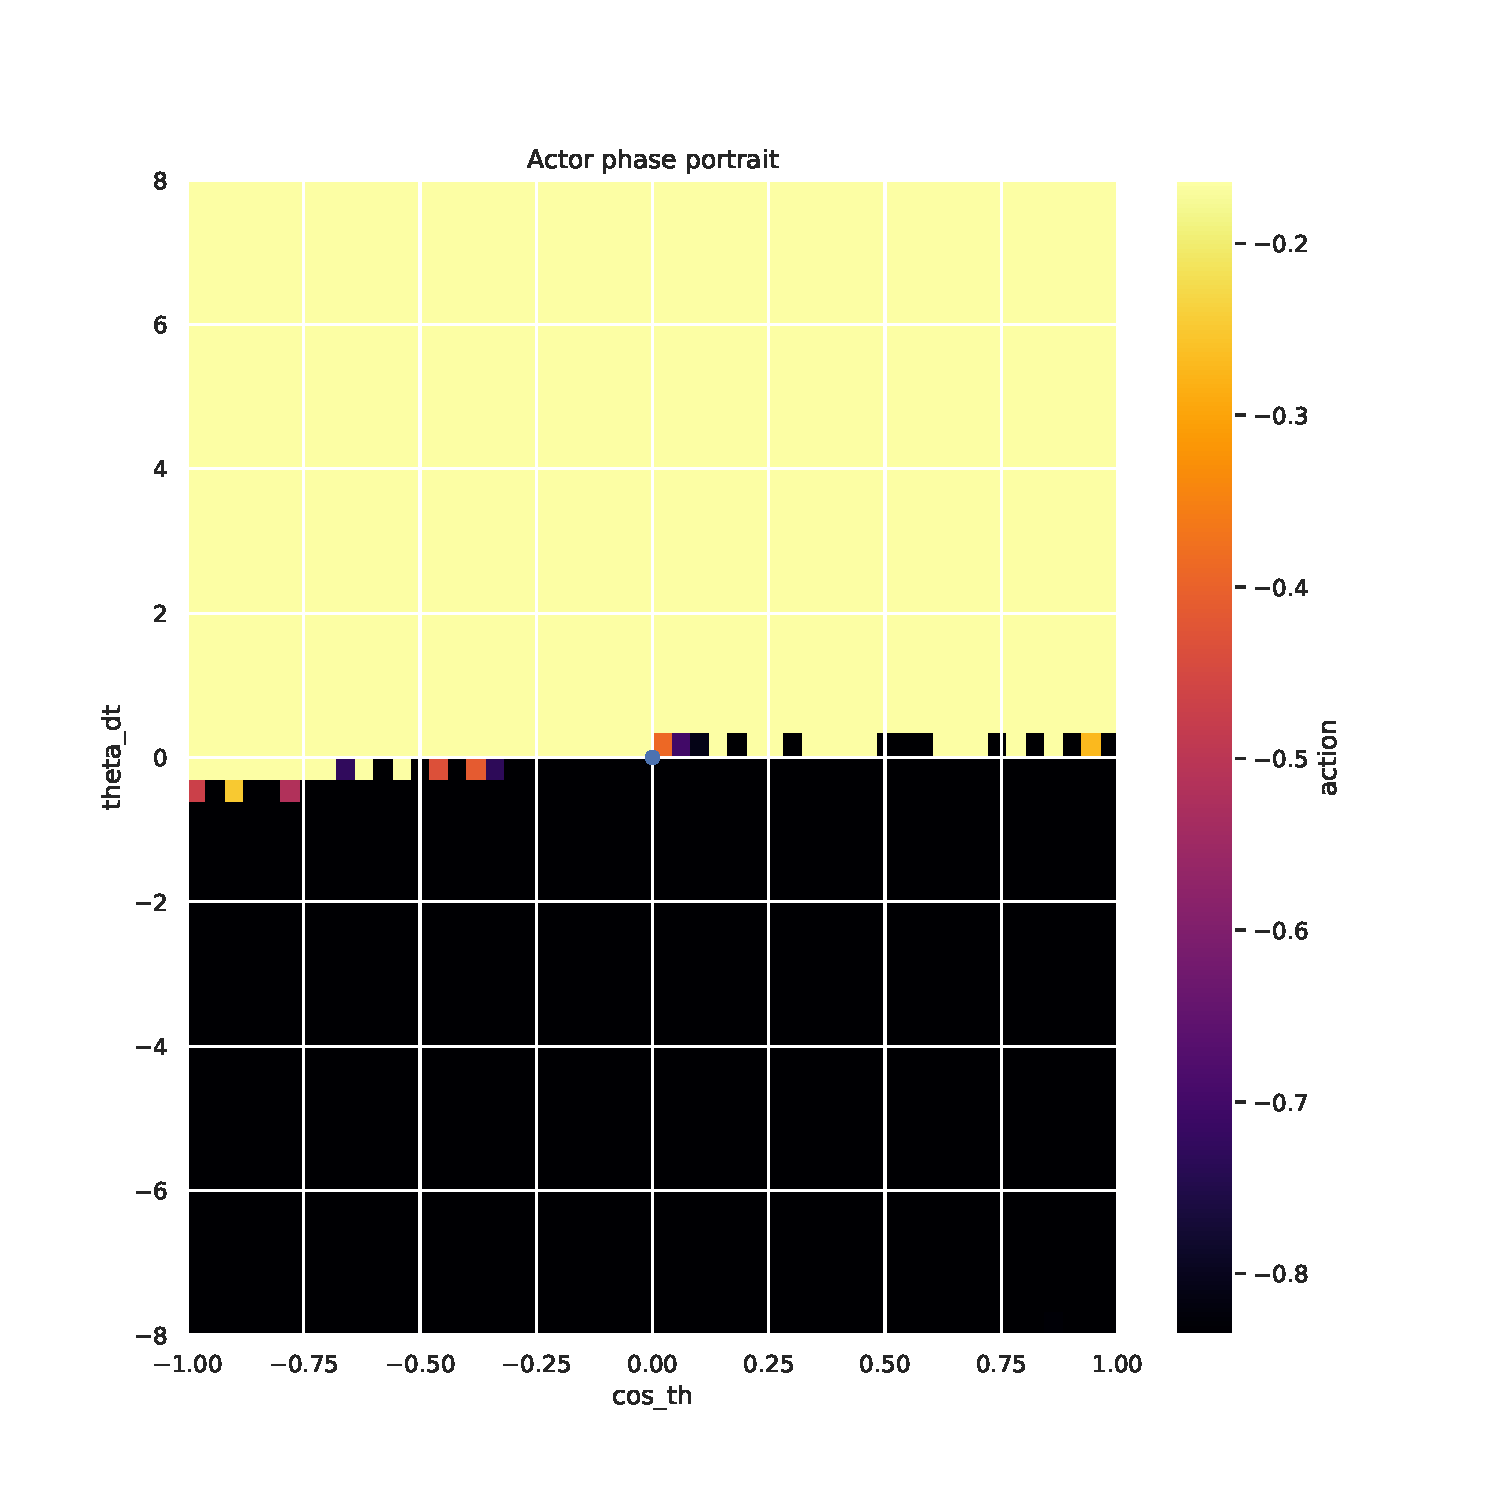
\includegraphics[width=\textwidth]{figures/iteration4/0_actor_normalize__post_Pendulum-v0.pdf}
        \caption{Acteur entraîné}
    \end{subfigure}
    \begin{subfigure}{0.3\textwidth}
        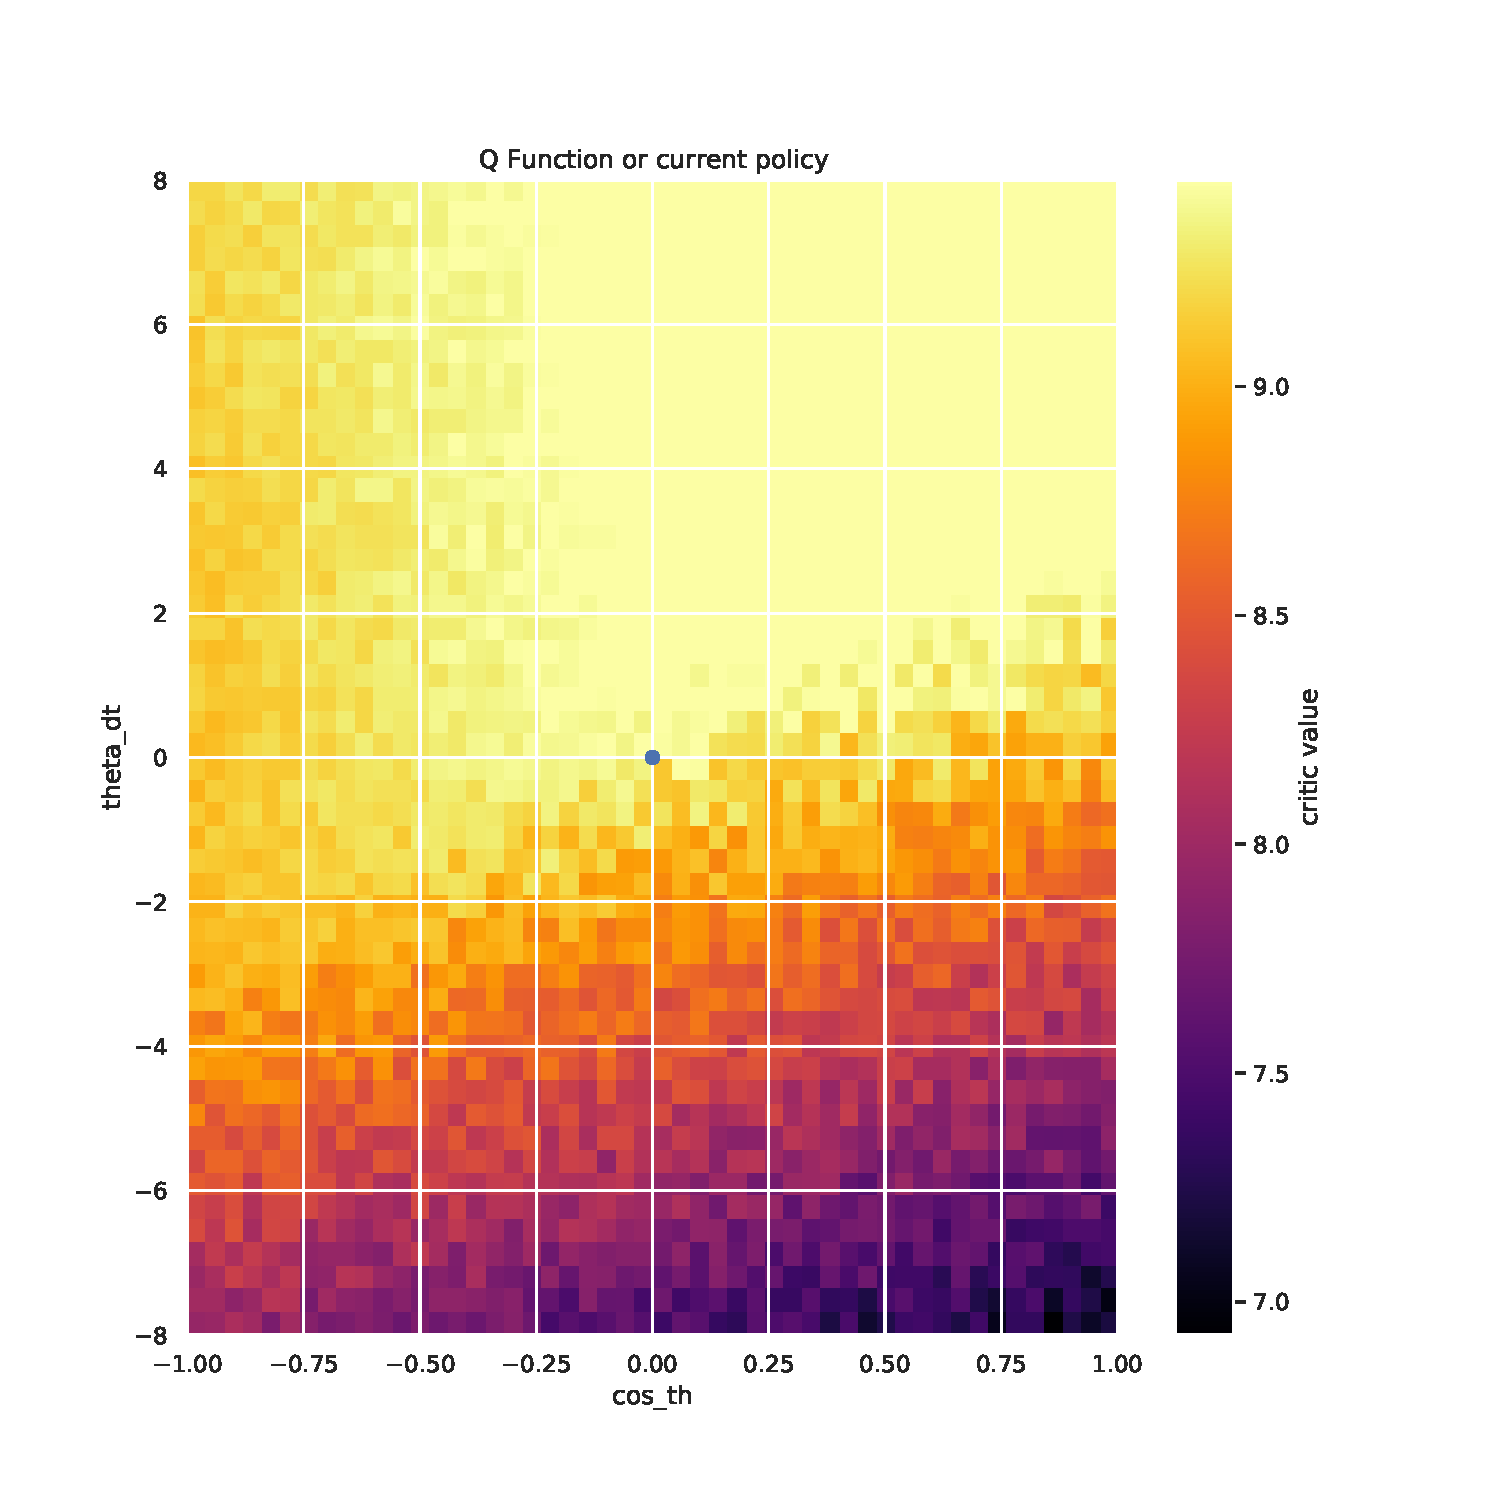
\includegraphics[width=\textwidth]{figures/iteration4/0_critic_normalize_post_Pendulum-v0.pdf}
        \caption{Critique entraînée}
    \end{subfigure}
    \caption{Valeurs de l'acteur et de la critique avec la méthode discount pour le calcul de la récompense}
    \label{fig:itr4_normalize}
\end{figure}

Ces graphes sur les figures~\ref{fig:itr4_discount} et \ref{fig:itr4_normalize} confirment que le problème ne vient pas de l'exploration mais plutôt de l'apprentissage en lui-même. Le problème est surement lié à l'implémentation. Puisque le projet contient un nombre conséquent de classes, nous n'approfondirons pas plus les recherches et nous implémentons un algorithme de \emph{policy grandient}.